\chapter{Proiectare de detaliu și implementare}
\pagestyle{fancy}

Acest capitol prezinta in detaliu solutia propusa pentru un sistem de monitorizare a temperaturii si a umiditatii. Aceasta include protocoalele de 
comunicatie utilizate, limbajele de programare si arhitecturi de abstractizare.

Arhitectura generala a sistemului este compusa din 5 componente pricipale interconectate pentru a crea o retea bine definita si cu o flexibilitate
ridicata:
\begin{enumerate}
	\item Aplicatie Android
	\item MQTT Broker
	\item Server
	\item Baza de date
	\item Senzor
\end{enumerate}

\

Figura \ref{fig:ArhitecturaGenerala} prezinta arhitectura generala a sistemului continand modulele principale ale acestuia si protocoalele de comunicatie 
dintre acestea.
\begin{figure}[H]
    \centering
    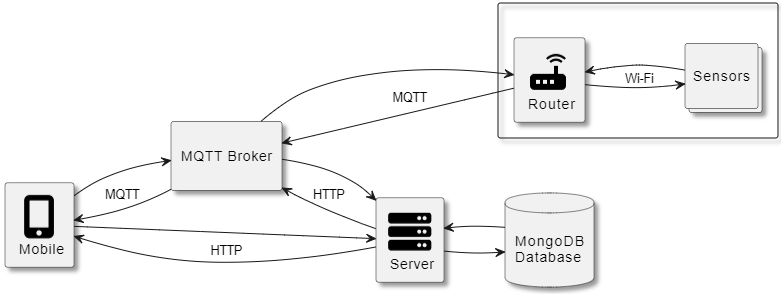
\includegraphics[scale=0.72]{figs/ArhitecturaGenerala.png}
    \caption{Arhitectura generala a proiectului}
    \label{fig:ArhitecturaGenerala}
\end{figure}

In intreaga retea este utilizat fusul orar UTC (Timpul Universal Coordonat) pentru a evita diferentele de fus orar local.

In subcapitolele urmatoare va fi descris in mod detaliat fiecare modul al sistemului si protocoalele de comunicatie utilizate pentru comunicarea dintre 
acestea.

\section{Aplicatia Android}\label{sec:pi_appandroid}
Aplicatia Android reprezinta interfata cu utilizatorul oferindui acestuia un mod usor de a gestiona mai multi senzori si de a monitoriza datele venite de la
acestia. Este scrisa in limbajul de programare Java si ruleaza pe sistemul de operare Android. Proiectul este scris in mediul de dezvoltare integrat Android 
Studio IDE.

In sistemul de operare Android clasele care definesc o interfata grafica sunt denumite activitati. La deschiderea aplicatiei este deschis firul de executie principal 
care are sarcina de a afisa interfetele grafice si de a gestiona actiunile utilizatorului, de exemplu, apasare de buton. Fiecare clasa de tip activitate extinde 
clasa AppCompatActivity care ofera componente pentru afisarea grafica si metode callback pentru gestionarea navigarii intre mai multe activitati. 

Aplicatia este compusa din 2 activitati principale si cateva secundare:
\begin{enumerate}
	\item ActivityWelcome - reprezinta activitatea care este afisata la deschiderea aplicatiei.
	\item ActivitySensor - reprezinta activitatea care este afisata atunci cand utilizatorul selecteaza un senzor din lista.
	\item ActivityInstall - reprezinta un grup de activitati secundare afisate atunci cand utilizatorul instaleaza un senzor nou. Fiecare dintre aceste 
	activitati reprezinta un pas din procesul de instalare.
\end{enumerate}

\

Figura \ref{fig:AndroidClassDiagram} prezinta diagrama de clase a aplicatiei Android.
\begin{figure}[H]
    \centering
    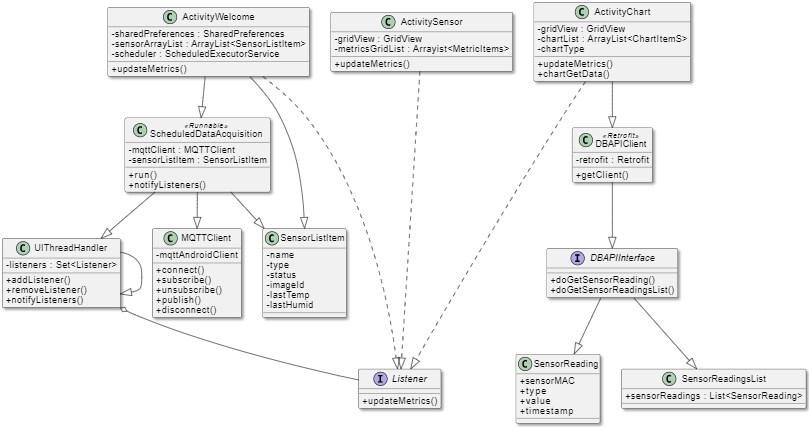
\includegraphics[scale=0.64]{figs/AndroidClassDiagram.png}
    \caption{Arhitectura generala a proiectului}
    \label{fig:AndroidClassDiagram}
\end{figure}

La incarcarea primei activitati care este afisata pe ecranul dispozitivului mobil, numita ActivityWelcome, se extrage din memorie o lista de senzori care au fost 
instalati in prealabil. Daca nu exista senzori instalati, aceasta lista nu va contine elemente. Lista este parcursa si pentru fiecare senzor este pornit un nou 
fir de executie periodic. Acest fir de executie are rolul de a gestiona conexiunea cu modulul MQTT Broker pentru senzorul respectiv, iar periodicitatea 
acestuia perimite verificarea si reincercarea conexiunii la un interval fix de timp. Apoi aceasta lista este afisata in interfata grafica. Fiecare element din lista 
contine: denumirea senzorului, tipul de senzor, statusul conexiunii si o imagine reprezentativa a senzorului.

Pentru memorarea senzorilor installati este utilizata biblioteca SharedPreferences. Aceasta contine rutine pentru salvarea datelor intr-un fisier din memoria 
dispozitivului mobil intr-un format de forma (cheie, valoare). Primul camp din acest fisier reprezinta numarul de senzori salvati, iar campurile ce urmeaza 
reprezinta senzorii instalati. Aceasta biblioteca este potrivita pentru memorarea datelor sub forma (cheie, valoare) si pentru compatibilitatea cu versiuni mai 
vechi de Android, spre deosebire de alte biblioteci precum DataStore care sunt potrivite pe seturi de date complexe si functioneaza doar in versiunile mai noi de 
Android.

Pentru firele de executie periodice este utilizata biblioteca ScheduledThreadPoolExecutor. Acesasta permite crearea unui grup de fire de executie care se executa
in paralel, spre deosebire de biblioteca Timer care are un singur fir de executie, iar o sarcina de durata mai lunga poate intarzia alte sarcini care asteapta 
executia. De asemenea, in cazul unei erori, doar sarcina in care a aparut eroarea va fi oprita, celelalte sarcini fiind executate in mod obisnuit. Aceasta 
biblioteca ofera siguranta continuarii executiei aplicatiei in cazul unei erori izolate.

La selectarea de catre utilizator a unui senzor din lista afisata este deschisa o noua activitate, numita ActivitySensor, iar la atingerea butonului de adaugare a unui 
nou senzor este deschisa prima activitate din grupul de activitati specifice instalarii. Pentru navigarea la o noua activitate si pentru transferarea de informatii intre 
activitati este utilizata clasa Intent. Aceasta clasa reprezinta o descriere abstracta a unei operatii. Cea mai semnificativa utilizare a acesteia este pentru operatia de 
deschidere a unei noi activitati. Pentru aceasta operatie se apeleaza functia startActivity() care primeste ca parametru o instanta a clasei Intent care contine informatiile 
necesare pentru ca operatia sa fie executata. Informatii precum activitatea parinte si activitatea care urmeaza a fi executata sunt necesare, iar in plus pot fi adaugate 
informatii care sa fie transferate catre activitatea copil utilizant functia putExtra() care primeste ca parametru o structura de tipul (cheie, valoare).

Pentru fiecare fir de executie specific unui senzor se creaza o instanta a clasei ScheduledDataAcquisition care implementeaza interfata runnable si executa periodic o rutina 
in care se verifica daca senzorul este conectat la modulul MQTT Broker. La prima executie senzorul este considerat deconectat si se executa rutina de conectare. 
Aceasta rutina utilizeaza clasa MQTTClient care ofera metodele necesare realizarii si gestionarii conexiunii cu modulul MQTT Broker. Pentru realizarea conexiunii se 
executa metoda connect a clasei MQTTClient care primeste ca paramterii 2 rutine callback. Aceste rutine definesc actiuni ce sunt executate atunci cand au loc 
diferite evenimente in tranzactionarea cu modulul MQTT Broker. Mai jos sunt enumerate cele mai importante astfel de evenimente:
\begin{itemize}
	\item Connectarea cu success la modulul MQTT Broker - cand are loc acest eveniment se executa rutina de subscriere pentru receptionarea in timp real a datelor de la 
	senzor.
	\item Pierderea conexiunii - acest eveniment va modifica statusul conexiunii din lista de senzori a-i activitatii ActivityWelcome si din ActivitySensor.
	\item Receptia unui mesaj - acest eveniment va apela metoda notifyListeners() a obiectului UIThreadHandler care va actualiza ultima valoare de temperatura si 
	umiditate afisata in activitatile ActivityWelcome si ActivitySensor. De asemenea, acest eveniment va verifica si statusul conexiunii senzorului si il va schimba 
	daca este cazul.
\end{itemize}

\

Clasa MQTTClient utilizeaza o instanta a clasei MqttAndroidClient oferita de biblioteca eclipse.paho.mqttv3 care reprezinta o implementare asincrona a 
al unui client al protocolului MQTT si are rolul de a gestiona impachetarea messajelor in formatul protocolului MQTT si tranzactionarea acestora cu un server MQTT. De asemenea, 
clasa MQTTClient defineste rutine de gestionare a exceptilor ridicate de obiectul MqttAndroidClient in cazul unei erori. 

Clasa UIThreadHandler are rolul de a efectua modificari in interfetele grafice de pe un fir de executie extern. Clasele de tip activitate sunt executate pe un fir de executie 
care are rolul strict de a raspunde la actiunile utilizatorului si doar acest fir de executie poate face modificari in interfata grafica, iar interogarea bazei de date sau 
receptionarea de date de la modulul MQTT sunt executate pe fire de executie diferite. Aceasta clasa realizeaza transferul de date sau evenimente care necesita modificarea 
interfetei grafice si care au fost primite pe un fir de executie extern catre firul de executie al interfetei grafice. Pentru a realiza acest transfer, instanta clasei  
UIThreadHandler mentine o lista de clase de tip Listener. Activitatile AvtivityWelcome si ActivitySensor sunt clase de tip Listener, deoarece implementeaza interfata 
Listener si metoda updateMetrics() a acesteia, iar la creare se inregistreaza in lista de obiecte Listener mentinuta de instanta UIThreadHandler. Fiecare activitate 
defineste in metoda updateMetrics() ce anume va fi modificat in interfata grafica. Atunci cand sunt receptionate date de la modulul MQTT Broker, se executa metoda 
notifyListeners() a obiectului UIThreadHander. Aceasta metoda parcurge lista de clase de tip Listener si pentru fiecare apeleaza metoda updateMetrics(). Aceasta metoda nu este 
apelata direct, ci prin obiectul Handler care primeste ca parametru o rutina de tip Runnable si care este pus intr-o coada de executie a interfetei grafice.

La selectarea unui element din lista de senzori afisata in activitatea ActivityWelcome este creata activitatea ActivitySensor. Rolul acesteia este de a prezenta informatiile 
senzorului selectat si datele de temperatura si umiditate ale acestuia sub forma grafica si sub forma a 2 campuri care contin doar ultima valoare receptionata. La creare 
se citeste din obiectul Intent primit de la activitatea ActivityWelcome informatiile senzorului intr-un obiect SensorListItem, se afiseaza informatiile senzorului in 
interfata grafica, se initializeaza graficele de temperatura si umiditate si se interogheaza baza de date pentru valorile din ultimele 10 minute. La primirea valorilor 
citite din baza de date, acestea sunt scrise in graficul de temperatura, respectiv umiditate. Daca nu exista date in ultimele 10 minute inseamna ca senzorul nu este conectat, iar 
statusul acestuia este modificat corespunzator. 

Pentru interogarea bazei de date este utilizata biblioteca Retrofit a carei functionalitate teoretica este descrisa in sectiunea \ref{sec:retrofit}. Pentru implementarea 
rutinelor de interogare a bazei de date utilizand aceasta biblioteca sunt utilizate urmatoarele clase din figura \ref{fig:AndroidClassDiagram}:
\begin{itemize}
	\item Clasa DBAPIClient - are rolul de a crea un obiect de tip Retrofit. Pentru crearea acestuia sunt necesare: adresa URL a server-ului, un obiect GsonConverterFactory 
	pentru convertirea automata a datelor si o instanta a clasei OkHttpClient.
	\item Interfata DBAPIInterface - declara metodele pentru interogarea bazei de date utilizand adnotari.
	\item Clasa SensorReading - este o clasa model care contine campurile receptionate in raspunsul metodei doGetSensorReading().
	\item Clasa SensorReadingsList - este o clasa model care contine o lista de obiecte de tip SensorReading. Aceasta lista reprezinta raspunsul metodei doGetSensorReadingsList().
\end{itemize}

La initierea unei interogari a bazei de date se obtine obiectul Retrofit utilizand metoda getClient() a clasei DBAPIClient. Se apeleaza metoda create() a obiectului Retrofit care 
primeste ca parametru interfata DBAPIInterface, iar pe baza acestei interfete, Retrofit va genera automat o clasa care contine implementarea metodelor declarate in aceasta. 
Utilizand instanta clasei creata automat se acceseaza una din metodele acesteia si se pune intr-o coada de transmisie impreuna cu o metoda callback care va fi executata cand 
este receptionat raspunsul de la server sau cand expira timpul de asteptare. La receptionarea raspunsului, biblioteca Retrofit va interpreta datele receptionate in format GSON 
bazat pe clasa model specifica metodei care s-a executat si va crea un obiect de acest tip. In metoda callback se citeste obiectul si se adauga valorile de temperatura si 
umiditate in graficul respectiv fiecareia. Pentru interpretare, a fost utilizat obiectul GsonConverterFactory care a fost instantiat la crearea obiectului Retrofit.

Pentru instalarea unui nou senzor, la apasarea butonului de adaugare din activitatea ActivityWelcome se deschide prima activitate din setul de activitati pentru instalare. 
Aceasta activitate cere utilizatorului inserarea datelor de conectare la senzor oferite in manualul de instalare. La apasarea butonului Next se deschide a activitatea de 
instalare specifica pasului doi in care se cere introducerea informatiilor router-ului prin care i se ofera senzorului access la internet. Al treila pas este reprezentat 
printr-o activitate care afiseaza durata si progresul procesului de instalare. La acest pas se realizeaza conexiunea completa a senzorului. La finalizeara conexiunii apare 
in activitate un buton care va redeschide activitatea ActivityWelcome, iar noul senzor adaugat va fi afisat in lista acesteia. 

\section{MQTT Broker}\label{sec:pi_mqttbroker}
Acest modul reprezinta punctul central al transmisiei in timp real al datelor achizitionate de senzor catre aplicatia Android.

Figura \ref{fig:MQTTBrokerInside} prezinta arhitectura interna a modulului MQTT Broker compusa din serverul MQTT Mosquitto oferit de organizatia Eclipse si o aplicatie 
Python.
\begin{figure}[H]
    \centering
    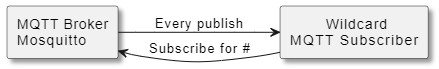
\includegraphics[scale=0.8]{figs/MQTTBrokerInside.png}
    \caption{Formatul datelor transmise de modulul MQTT Broker catre Android}
    \label{fig:MQTTBrokerInside}
\end{figure}

Modulul Mosquitto MQTT Broker este instalat pe o masina virtuala cu un sistem de operare linux utilizand comanda "sudo apt-get install mosquitto mosquitto-clients -y". 
In mod implicit acesta este configurat sa comunice pe portul 1883, dar poate fi modificat accesand fisierul de configurare "/etc/mosquitto/mosquitto.conf". Pentru 
pornirea serverului trebuie executata comanda "sudo systemctl start mosquitto", iar pentru pornirea automata la deschiderea sistemului de operare linux se executa 
comanda "sudo systemctl enable mosquitto".

Modulul Wildcard MQTT Subscriber este o aplicatie scrisa in limbajul de programare Python care are rolul de a intercepta toate mesajele care ajung in Broker de la dispozitivele 
cu rol de publicator si de a le transmite catre modulul RESTful Server pentru memorarea acestora in baza de date. In structura unei retele MQTT, aceasta aplicatie are un rol 
special de abonator pentru toate mesajele de date care ajung in Broker de la publicatori. Pentru a realiza aceasta abonare, aplicatia trimite o cerere de abonare catre 
Broker pentru topicul "readings/\#" care specifica abonarea pentru toate topicurile care incep cu "readings/" si contin orice altceva in rest '\#'. Mesajele de configurare 
sau alarmele transmise intre aplicatia Android si senzor nu vor fi interceptate de acest abonator, doarece topicurile respective incep cu sirul de caractere "config/" sau 
"alarm/".

Pentru implementarea aplicatiei Python este utilizata biblioteca "paho.mqtt.cient". Aceasta ofera rutine ajutatoare pentru crearea unui client cu rol de abonator sau publicator 
intr-o retea MQTT. De asemenea, ofera rutine de callback care permit realizarea anumitor actiuni atunci cand au loc evenimente precum receptia unui mesaj, connectarea cu 
success, subscriptia cu success etc. La receptia unui mesaj de la Broker se creeaza o cerere HTTP cu metoda POST care este transmisa catre modulul RESTful Server pentru 
salvarea datelor in baza de date. De la senzor se primeste metrica si valoarea acesteia intr-un format JSON, \ref{fig:Mqtt2AndroidDataFormat} prezinta acest format. Este de 
datoria aplicatiei sa extraga adresa MAC a senzorului din topic si sa adauge o unitate de timp in fus orar UTC la datele receptionate inainte de transmisia lor catre baza de 
date.

Figura \ref{fig:Mqtt2AndroidDataFormat} prezinta formatul JSON al datelor transmise de catre senzor si retransmise de catre Broker inspre aplicatia Android si baza de date. 
Sunt trimise 2 mesaje separate, unul pentru temperatura si unul pentru umiditate. 
\begin{figure}[H]
    \centering
    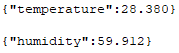
\includegraphics[scale=0.8]{figs/Mqtt2AndroidDataFormat.png}
    \caption{Formatul datelor transmise de modulul MQTT Broker catre Android}
    \label{fig:Mqtt2AndroidDataFormat}
\end{figure}

\section{RESTful Server}\label{sec:pi_restserver}
Modulul RESTful Server reprezinta punctul de legatura intre aplicatia Android si baza de date si intre modulul MQTT Broker si baza de date. Acesta este implementat in limbajul 
de programare Python si utilizeaza biblioteca Flask. Pentru comunicarea cu acesta este utilizat protocolul HTTP. 

Figura \ref{fig:PI_RealFlaskProjectStructure} prezinta structura fisierelor proiectului Python utilizand Flask. 
\begin{figure}[H]
    \centering
    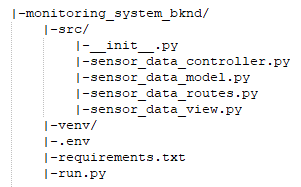
\includegraphics[scale=0.9]{figs/PI_RealFlaskProjectStructure.png}
    \caption{Arhitectura generala a proiectului}
    \label{fig:PI_RealFlaskProjectStructure}
\end{figure}

Structura fisierelor proiectului respecta structura de baza a unui proiect Python utilizand Flask descrisa in sectiunea \ref{sec:flask}. De asemenea, respecta si 
modularizarea codului sursa conform modelului arhitectural MVC, Model-View-Controller. In urmatoarele paragrafe se va descrie fiecare modul continut in directorul 
src/ si care sunt functiile acestora.

Fisierul sensor\_data\_routes.py reprezinta punctul de intrare in aplicatie. Acesta contine o corelare intre adresele URL pe care server-ul le cunoaste si clasele model 
sub forma de resurse. O adresa URL identifica unic o resursa sau o clasa model. Orice cerere HTTP care vine din retea, de la aplicatia Android sau de la modulul MQTT Broker, 
vor fi validate in acest modul pe baza andresei URL.

Fisierul sensor\_data\_controller.py reprezinta punctul de control al aplicatiei. Acesta primeste de la modulul Routes resursa care se doreste a fi accesata din baza de date, 
identifica metoda HTTP si argumentele acesteia, valideaza aceste informatii si transmite catre modulul Model interogarea specifica resursei. La returnarea datelor de catre 
modulul Model, acesta va transmite catre modulul View datele receptionate pentru a fi formatate corespunzator, iar apoi va transmite raspunsul catre entitatea care a transmis 
cererea.

Fisierul sensor\_data\_model.py reprezinta modulul Model al aplicatiei. Acesta contine implementarea propriu-zisa a metodelor de interogare a bazei de date. Exista o metoda 
specifica fiecarei resurse pentru a facilita dezvoltarea ulterioara si optimizarea interogarilor catre baza de date.

Fisierul sensor\_data\_view.py reprezinta modulul View al aplicatiei. Acesta are rolul de a formata datele extrase din baza de date in formatul pe care entitatea care a 
efectuat cererea il cunoaste, si anume formatul GSON. 

Figura \ref{fig:Server2AndroidDataFormat} prezinta formatul JSON al datelor trimise catre aplicatia Android de la modulul Server in urma unei interogari a bazei de 
date pentru valorile de umiditate dintr-o anumita perioada. Raspunsul prezentat contine o lista cu 3 citiri diferite.
\begin{figure}[H]
    \centering
    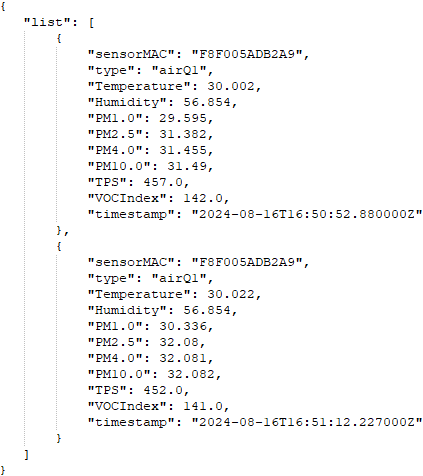
\includegraphics[scale=0.8]{figs/Server2AndroidDataFormat.png}
    \caption{Exemplu de raspuns la o interogare a bazei de date}
    \label{fig:Server2AndroidDataFormat}
\end{figure}

O problema bine cunoscuta a bibliotecii datetime din limbajului de programare Python si care a fost intampinata la formatarea datelor in modulul View este fusul orar. 
Atunci cand un sir de caractere este convertit in formatul datetime sau invers, acesta nu contine informatii legate de fusul orar, UTC sau local. Sirul de caractere 
'2024-06-16T11:23:53.015001Z' va fi interpretat ca un obiect de tipul datetime din care informatia 'Z', care reprezinta fusul orar UTC, este pierduta. 
Trebuie specificat explicit ce fus orar este utilizat la apelul functiei de convertire. Atunci cand este specificat fusul orar, sirul de caractere 
'2024-06-16T11:23:53.015001Z' va fi interpretat ca un obiect datetime din care informatia 'Z' este inlocuita cu '+00:00'. Ambele siruri, 'Z' si '+00:00' semnifica fus orar 
UTC, dar nu toate librariile din alte limbaje de programare interpreteaza corect sirul de caractere '+00:00'. In biblioteca Retrofit, modulul care mapeaza automat un sir de 
caractere in format GSON pe o clasa model nu interpreteaza corect sirul '+00:00'. Pentru a rezolva aceasta problema, in modulul View, a fost necesara inlocuirea manuala a sirului 
de caractere '00:00' cu 'Z'. O alta rezolvare a acestei problema ar fi fost scrierea manuala a codului pentru maparea datelor pe o clasa model in loc de utilizarea uneia deja 
existente in biblioteca Retrofit. 

\section{Baza de date MongoDB}\label{sec:pi_bazadedate}
Acest modul are rolul de a memora datele transmise de catre senzori si de a facilita extractia acestora la cererea utilizatorilor. Acesta comunica prin intermediul 
protocolului de comunicatie TCP/IP Sockets cu serverul RESTful, acesta din urma reprezentand interfata de comunicare dintre modulele MQTT Broker si Mobile cu baza 
de date. 

Baza de date MongoDB ofera un mod eficient si optimizat de memorare a datelor care contin o unitate de timp, numit Time Series Collection. Acest lucru face ca aceasta 
baza de date sa fie cea mai potrivita pentru proiectele din domeniul IoT in care momentul de timp la care datele sunt colectate este foarte important.

Figura \ref{fig:PI_MongodbDocExample} prezinta structura unui document memorat in baza de date. 
\begin{figure}[H]
    \centering
    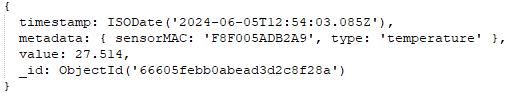
\includegraphics[scale=0.8]{figs/PI_MongodbDocExample.png}
    \caption{Exemplu de document din baza de date}
    \label{fig:PI_MongodbDocExample}
\end{figure}

Aceasta baza de date este formata dintr-o colectie numita "readings" care contine mai multe documente. Un document reprezinta datele pe care un sezor le-a achizitionat 
la un moment de timp. Structura unui document contine urmatoarele campuri:
\begin{itemize}
	\item Campul "timestamp" - reprezinta unitatea de timp la care datele au fost achizitionate de catre senzor. Aceasta unitate de timp contine an, luna, zi, ora, 
	minut, secunda si milisecunda. Formatul unitatii de timp trebuie sa respecte standardul international ISO, care defineste ordinea parametrilor de timp, 
    fusul orar si caracterele utilizate pentru delimitarea acestora.
	\item Campul "metadata" - reprezinta informatii despre senzor si despre datele continute in document. Acest camp ar trebui sa contina elemente care se schimba 
	foarte rar sau niciodata. De asemenea, elementele pe baza carora se fac interogarile in baza de date trebuie sa fie continute in acest camp pentru a beneficia 
    de eficienta maxima. Acest camp contine adresa MAC a senzorului si tipul metricii venite de la senzor. 
	\item Campul "value" - reprezinta valoarea metricii venita de la senzor. De exemplu, temperatura in grade celsius.
	\item Campul "\_id" - reprezinta un sir de caractere generat automat la memorarea documentului care identifica unic acest document.
\end{itemize}

Figura \ref{fig:PI_AggregationExample} prezinta operatia de agregare utilizata pentru extragerea documentelor care se afla intr-un anumit interval de timp. Prima 
operatie efectuata este "\$match" care va selecta din baza de date toate documentele care se afla intr-un anumit interval de timp. A doua operatie efectuata este 
tot operatia "\$match" care va selecta din documentele care au indeplinit conditia primei operatii, doar documentele caare au o anumita adresa MAC si care contin 
un anumit tip de valori, cum ar fi valori de umiditate. A treia operatie este "\$sort" care va aranja documentele care au indeplinit conditiile celei de-a doua 
operatii in ordine cronologica. Ordinea acestor operatii este foarte importanta pentru cresterea eficientei. S-a ales operatia de selectare a intervalului de timp 
ca prima operatie, deoarece este operatia cea mai putin costisitoare de efectuat pe intreaga baza de date. Astfel, setul de documente pe care se efectueaza celelalte 
doua operatii, care sunt mult mai costisitoare, este diminuat semnificativ.
\begin{figure}[H]
    \centering
    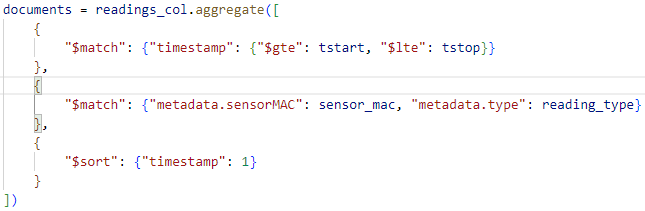
\includegraphics[scale=0.8]{figs/PI_AggregationExample.png}
    \caption{Exemplu de operatie de agregare}
    \label{fig:PI_AggregationExample}
\end{figure}

\section{Senzor}\label{sec:pi_senzor}
Acest modul este compus din doua componente principale, un dispozitiv care are capabilitatile de a esantiona date de temperatura si umiditate si de a comunica 
printr-un mediu fara fir si un router care realizeaza legatura dintre reteaua locala si internet. Rolul acestui modul este de a realiza o conexiune cu un router,
de a achizitiona date de temperatura si umiditate si de a le transmite catre aplicatia Android. 

Pentru realizarea senzorului s-a utilizat platforma de dezvoltare Arty Z7 la care este conectat un controller de retea ATWINC1500 si senzorul de temperatura 
si umiditate HDC1080. Pentru realizarea schemei arhitecturale a fost utilizat mediul de dezvoltare Xilinx Vivado 2018.3, iar pentru dezvoltarea codului sursa 
in limbajul de programare C a fost utilizat mediul de dezvoltare Xilinx SDK 2018.3.

Figura \ref{fig:PI_SensorUnitDiagram} prezinta arhitectura modulului de achizitionare de temperatura si umiditate.
\begin{figure}[H]
    \centering
    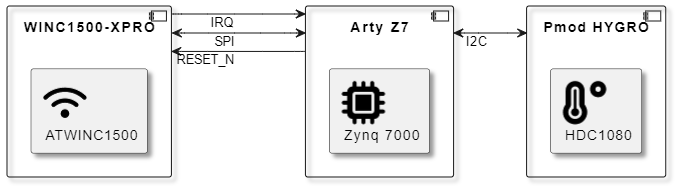
\includegraphics[scale=0.8]{figs/PI_SensorUnitDiagram.png}
    \caption{Arhitectura senzorului de temperatura si umiditate}
    \label{fig:PI_SensorUnitDiagram}
\end{figure}

\subsection{Platforma de dezvoltare Arty Z7}\label{subsec:artyz7_platform}
Nucleul platformei de dezvoltare Arty Z7 este sistemul integrat Zynq7000, avand o multitudine de porturi si componente periferice pentru adaptarea la diferite 
priecte. De pe aceasta platforma sunt utilizate cele doua porturi pmod pentru conectarea senzorului HDC1080 si a controllerului de retea ATWINC1500, sistemul 
integrat Zynq7000 reprezentand unitatea de control al tututor perifericelor de pe platforma si portul MicroUSB utilizat pentru alimentarea cu 5 volti si pentru 
comunicatia cu un calculator personal prin interfata de comunicare UART.

Arhitectura interna a sistemului integrat Zynq7000 este formata dintr-un procesor de tip ARM Cortex-A9 cu doua nuclee si partea logica FPGA 7-series. Proiectul 
de fata utilizeaza procesorul ARM Cortex-A9 pentru crearea unui microcontroller si partea logica pentru conectarea porturilor necesare la microcontroller. 

Schema de design a platformei Arty Z7 contine un set de periferice si porturi care sunt conectate la procesorul ARM Cortez-A9 si un set de periferice si porturi 
conectate la partea logica FPGA. De exemplu, porturile pmod sunt conectate la partea logica, iar portul MicroUSB este conectat la procesor. Pentru utilizarea 
componentelor sau porturilor periferice conectate la partea logica FPGA in procesorul ARM Cortex-A9 este utilizata interfata EMIO care este o extensie a 
multiplexorului de intrari si iesiri al procesorului.

Figura \ref{fig:PI_ZynqBlockDesign} prezinta interconexiunea dintre procesor si porturile periferice.
\begin{figure}[H]
    \centering
    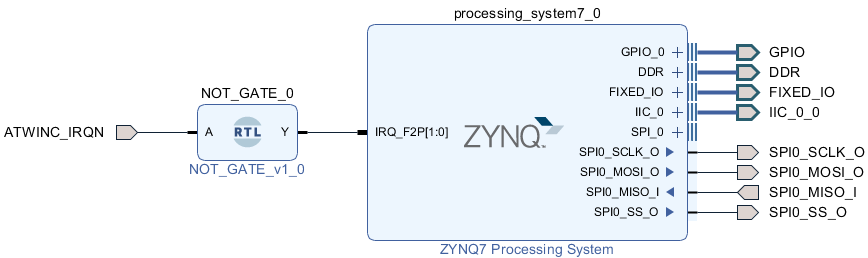
\includegraphics[scale=0.68]{figs/PI_ZynqBlockDesign.png}
    \caption{Diagrama de proiectare}
    \label{fig:PI_ZynqBlockDesign}
\end{figure}

Portul "ATWINC\_IRQN" reprezinta semnalul de intrerupere al controllerului de retea ATWINC1500 activ in 0 logic. Acesta este conectat la o poarta NU pentru a 
inversa polaritatea semnalului, deoarece unitatea generala de control al intreruperilor (GIC) nu are polaritate configurabila. Acesta genereaza o intrerupere 
doar la tranzitia din 0 logic in 1 logic. Porturile a caror denumire incep cu "SPI0" reprezinta semnalele protocolului SPI utilizate in comunicarea cu controllerul 
de retea ATWIN1500, iar portul "GPIO" reprezinta semnalul de reset al modulului ATWINC1500 care, la fel ca semnalul de intrerupere, este activ in 0 logic. Aceste 
semnale sunt legate la portul PMODA (JA) de pe platforma Arty Z7.

Portul "IIC\_0\_0" reprezinta semnalele protocolului I2C utilizat in comunicatia cu senzorul de temperatura si umiditate HDC1080. Aceste semnale sunt legate pe 
portul PMODB (JB) de pe platforma Arty Z7.

Porturile "DDR" si "FIXED\_IO" sunt generate automat la crearea unitatii de procesare. Portul "DDR" realizeaza conexiunea dintre procesorul ARM Cortex-A9 si memoria 
externa DDR utilizata la incarcarea si executarea codului sursa, iar portul "FIXED\_IO" reprezinta semnalele de intrare/iesire ale perifericelor utilizate. De exemplu 
semnalele conectate intre interfata UART si portul microUSB.

Pentru creearea diagramei de proiectare in mediul de lucru Vivado 2018.3 sunt necesari urmatorii pasi descrisi succint:
\begin{enumerate}
	\item Se creeaza un proiect nou selectand sistemul integrat Zynq7000.
	\item Din meniul "IP Integrator" se creeaza un nou bloc de design.
	\item Prin apasarea butonului "Add IP" din fereastra design-ului se adauga procesorul Zynq7000.
	\item Prin dublu click pe blocul nou aparut al procesorului se deschide meniul de configurare al acestuia. Din acest meniu se selecteaza sursa de ceas si frecventa 
	acestuia, liniile de intrare iesire si perifericele utilizate.
    \item La apasarea butonului "OK" vor aparea pe blocul procesorului toate perifericele care se conecteaza la o componenta externa.
    \item Crearea porturilor externe se face prin click dreapta pe diagrama si "Create port". Acestuia i se atribuie un nume, o directie si un tip.
    \item Pe baza diagramei create Vivado va genera automat instructiunile necesare maparii porturilor prin click dreapta pe fisierul designului si "Create HDL Wrapper".
    \item Se genereaza sirul de biti pentru partea logica FPGA prin apasarea butonului "Generate Bitstream".
    \item Se exporta diagrama si sirul de caractere intr-un fisier pe care mediul de dezvoltare Xilinx SDK il va interpreta si va genera driverele necesare. Acest 
    fisier contine informatiile necesare generarii driverului doar pentru perifericele activate si configurate la pasul 4.
\end{enumerate}

Platforma de dezvoltare Arty Z7 ofera ca sursa de ceas un crystal cu frecventa de 50 MHz care este conectat ca intrare in procesorul ARM Cortex-A9. Procesorul multiplica 
semnalul de ceas printr-un circuit PLL, iar apoi il distribuie componentelor periferice. Alegerea frecventei sursei de ceas este in stransa legatura cu modulele timer 
necesare functionarii aplicatiei, si anume, doua module timer care numara la milisecunda. Pentru a obtine o acuratete cat mai buna a milisecundei, sursa de ceas este 
multiplicata cu un factor de 16, obtinand astfel o frecventa a sursei de ceas de 400Mhz.

Figura \ref{fig:PI_SDKFileStructure} prezinta structura fisierelor proiectului in mediul de programare Xilinx SDK. Fiecare director reprezinta un modul al proiectului 
si contine fisere asociate cu denumirea acestuia.
\begin{figure}[H]
    \centering
    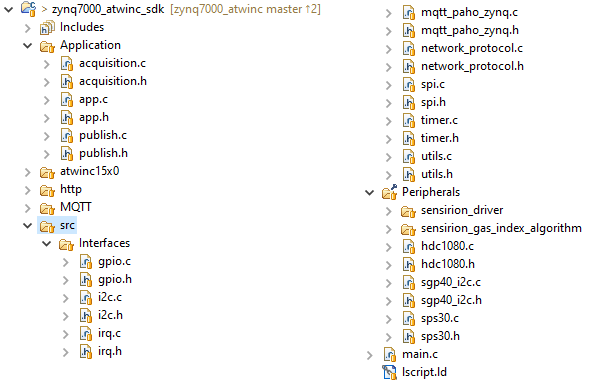
\includegraphics[scale=0.66]{figs/PI_SDKFileStructure.png}
    \caption{Structura fisierelor proiectului}
    \label{fig:PI_SDKFileStructure}
\end{figure}

Driverul generat automat de catre mediul de dezvoltare Xilinx SDK se afla intr-un proiect separat numit "Zynq7000\_atwinc\_sdk\_bsp". Acest proiect este generat automat 
bazat pe fisierul ".hdf" exportat de mediul de dezvoltare Vivado.

Directorul "MQTT" contine rutinele necesare crearii si mentinerii unei conexiuni cu un Broker MQTT si formatarea pachetelor conform acestui protocol. Implementarea 
driverului este oferita de organizatia Eclipse cu liceta deschisa si poate fi descarcat sub forma de arhiva de pe github. Acest driver este impartit in doua directoare, 
"MQTTClient-C" si "MQTTPacket". Directorul "MQTTClient-C" contine rutinele necesare crearii si mentinerii conexiunii, iar "MQTTPacket" contine rutine pentru serializarea 
diferitelor pachete specifice protocolului MQTT. Fisierul antet din directorul "MQTTClient-C" contine declaratii externe ale rutinelor de scriere si citire a unui pachet si 
ale rutinelor pentru managementul timerelor care sunt specifice fiecarei platforme si trebuie implementate de catre integratorul driverului. Driverul este compatibil cu 
mai multe platforme, Linux, Windows, EmbeddedOS sau Embedded. Functionalitatea oferita pentru platforma Embedded este bazata pe asteptare ocupata, firul de executie 
este blocat pentru asteptarea raspunsului pentru un anumit pachet, care este o practica contraindicata in sistemele embedded. Avand in vedere acest lucru, fisierele 
din directorul "MQTTClient-C" au fost modificate astfel incat sa nu mai blocheze firul de executie. Modificarile constau in inlocuirea zonelor de cod unde se asteapta 
receptionarea unui raspuns la pachetul transmis sau expirarea timpului acordat pentru operatia curenta cu o variabila de stare si un modul timer global care este 
verificat periodic la frecventa rularii buclei principale. Variabila de stare contine statusul curent al modulului MQTT, operatie in derulare sau liber pentru 
o noua operatie si functioneaza ca un semafor, daca exista o operatie in derulare nu se va initia o noua operatie si la urmatoarea executie a buclei principale se va 
verifica din nou daca este posibila initierea noii operatii. Timerul global se asigura ca daca o operatie in derulare nu ofera nici un raspuns intr-o perioada 
predefinita, acesta va executa rutinele necesare rezolvarii erorii care a dus la pierderea operatiei. La rutinele din directorul "MQTTPacket" nu au fost ecesare 
modificari, fiind complet decuplate de platforma de executie. 

Directorul "ATWINC15x0" reprezinta driverul pentru controlerul ATWINC1500 oferit de organizatia Microchip sub licenta libera. Driverul este inclus in libraria 
"mla", Microchip Libraries for Applications, si poate fi descarcat de pe site-ul oficial al organizatiei Microchip. Acesta este descris in detaliu in subcapitolul
\ref{subsec:atwinc1500}.

Directorul "Interfaces" reprezinta o abstractizare a driverelor utilizate in proiect, Zynq driver, ATWINC1500 driver si MQTT driver. Fiecare fisier sursa din acest director 
contine rutine pentru initializarea perifericului specific denumirii fisierului si rutine pentru controlul acestuia. De asemenea, in cazul perifericelor care functioneaza 
bazat pe intreruperi fisierul contine si rutinele de tip Handler care se executa la aparitia unui eveniment. Fisierele antet contin macrouri pentru caracteristicile 
fiecarui periferic, macrouri pentru identificarea pinilor sau pentru functii care pot fi sicrise intr-o singura linie de cod, si declaratii ale rutinelor care sunt 
utilizate de fisiere externe. Fisierele utils.c si utils.h contin rutine generale utile intr-un proiect, cum ar fi o rutina pentru blocarea executiei pentru o anumita 
perioada de timp (BusyDelay) si rutine pentru conversii intre tipuri de veriabile, de exemplu conversia din float in string sau inversarea ordinii caracterelor intr-un 
string. Fisierele "netwrok\_protocol.c" si "network\_protocol.h" abstractizeaza operatiile necesare pentru initializarea si crearea unui Socket si pentru conectarea 
la server.

Directorul "Application" contine fisiere sursa si antet specifice aplicatiei. Fisierul "acquisition.c" contine rutine pentru initializarea si gestionarea achizitiei 
de date de la senzorul de temperatura si umiditate HDC1080. Acesta contine o masina de stari care initiaza o noua achizitie de date, asteapta finalizarea acesteia, 
converteste valorile obtinute in sir de caractere si gestioneaza posibilele erori. Fisierul "acquisition.h" contine declaratia starilor masinii de stari si a 
variabilelor si functiilor utilizate de fisiere externe. Fisierul "publish.c" este responsabil cu calcularea urmatorului moment in care se va transmite un pachet,
de creearea pachetului si adaugarea acestuia in coada. Fisierul "app.c" contine masina de stare generala a aplicatiei, functii de tip handler care gestioneaza 
evenimentele care au loc in retea, masina de stare pentru resetarea dispozitivului la setarile din fabrica si defineste o coada de mesaje si rutinele necesare 
pentru gestiunea acesteia, adaugare pachet, extragere pachet, stergere pachet. 

Directorul "Peripherals" contine fisierele specifice fiecarui periferic al platformei Zynq Z7, controlerul de retea ATWINC1500 si senzorul de temperatura si 
umiditate HDC1080. Fisierele "hdc1080.c" si "hdc1080.h" definesc rutinele pentru initializarea si configurarea modulului HDC1080. De asemenea, contine si o masina 
de stare pentru inceperea unei esantionari de date si citirea acestora. Fisierul "winc1500\_api.c" reprezinta fisierul in care sunt implementate functiile de tip 
stub specifice modulului ATWINC1500.

Fisierul lscript.ld reprezinta fisierul care defineste adresa de baza a memoriei unde este scris codul sursa, dimensiunea memoriilor RAM si dimensiunea stivei.

Figura \ref{fig:PI_MainStateMachine} prezinta principalele sarcini si evenimente ale senzorului.
\begin{figure}[H]
    \centering
    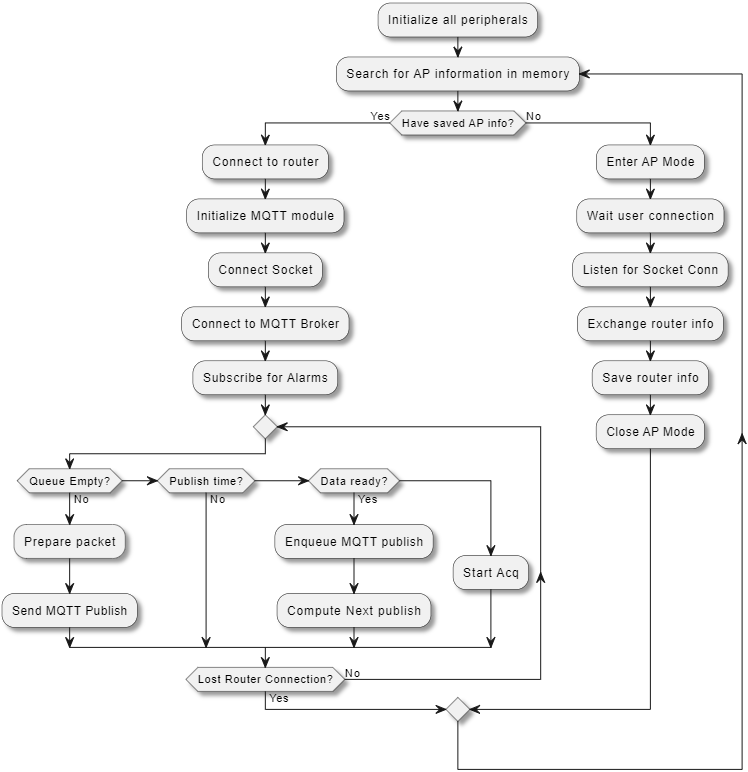
\includegraphics[scale=0.66]{figs/PI_MainStateMachine.png}
    \caption{Masina de stare principala}
    \label{fig:PI_MainStateMachine}
\end{figure}

Urmatoarele paragrafe contin o descriere a fluxului de executie prezentat in figura \ref{fig:PI_MainStateMachine} cu accentul pe functionalitatile care nu au putut 
fi cuprinse in figura din cauza complexitatii si a dimensiunii. 

La pornirea sistemului este executata starea "Initialize all peripherals" unde sunt initializate toate perifericele utilizate de catre aplicatie, atat cele externe 
platformei Arty Z7, modulul HDC1080 si modulul ATWINC1500, cat si cele integrate, modulele Clock, Timer, Interrupts etc.

La pornirea buclei infinite este executata starea "Search for AP information in memory" in care se verifica daca modulul ATWINC1500 contine in memorie informatiile 
necesare pentru conectarea la un router. Aceste informatii sunt numele retelei (SSID), tipul de autentificare si parola, fiind memorate la finalul procesului de instalare. 
Daca nu exista informatii salvate in memorie, se va executa ramura din dreapta a figurii \ref{fig:PI_MainStateMachine}, ramura "Nu" a conditiei "Have saved AP info?". 
Aceasta ramura prezinta pasii care sunt executati in procesul de instalare al senzorului.

Procesul de instalare al senzorului incepe cu starea "Enter AP Mode" unde modulul ATWINC1500 intra in starea de AP (Access Point). In aceasta stare dispozitivul 
functioneaza ca un router care accepta o singura conexiune. Apoi, in starea "Wait user connection", modulul ATWINC1500 asteapta ca aplicatia Android sa se conecteze 
la el. Dupa realizarea conexiunii se executa starea "Listen for Socket Conn" unde modulul ATWINC1500 creeaza un socket si asteapta ca aplicatia Android sa se conecteze 
la acest socket pentru a putea comunica. Dupa realizarea conexiunii la socket, in starea "Exchange router info" senzorul primeste informatiile necesare pentru conectarea 
la un router. Aceste informatii sunt salvate in memorie in starea "Save router info", iar apoi se intra pe fluxul de executie al cazului in care informatiile routerului 
exista in memorie.

In starea "Connect to router" este realizata conexiunea senzorului la router bazat pe informatiile din memorie. 

Dupa conectarea cu succes la router este executata starea "Initialize MQTT module" unde este initializat driverul MQTT. In aceasta stare se aloca zonele de memorie 
utilizate pentru transmisia si receptia de pachete si timpul de asteptare pentru receptia unui raspuns.

In starea "Connect Socket" se creeaza un canal de comunicatie si se realizeaza conexiunea cu masina pe care ruleaza Brokerul MQTT.

Dupa conectarea cu success la platforma in care ruleaza Brokerul MQTT, in starea "Connect to MQTT Broker", se realizeaza conexiunea cu acesta prin transmiterea 
pachetului MQTT CONNECT.

In starea "Subscribe for alarms" senzorul transmite un mesaj Brokerului MQTT prin care cere subscriptia la topicul pentru configurari. Acest topic este utilizat pentru 
receptia de mesaje de configurare de la aplicatia Android.

Daca in oricare din starile care presupun o conexiune cu un modul extern are loc o eroare se va aplica un algoritm de crestere a timpului intre reincercari 
exponential. Acest algoritm incepe cu o reincercare imediata, apoi va reincerca conexiunea dupa 10 secunde, dupa 30 de secunde, dupa un minut si in final la fiecare 
5 minute. Acest algoritm previne reincercarea conexiunii prea frecvente care poate duce la supraincarcarea modulului extern.

Urmatoarea stare este ilustrata prinytr-un romb gol care semnifica inceperea buclei de functionare a aplicatiei. Cat timp senzorul functioneaza normal, nu se pierde 
conexiunea cu oricare din modulele externe sau nu este actionat fizic de catre utilizator, aceasta va executa aceasta bucla la infinit. In aceasta bucla, in starea 
"Queue Empty?" se verifica daca exista un mesaj in coada de aplicatie. Daca exista un mesaj acesta este transmis, iar daca nu exista se trece mai departe si se verifica, 
in starea "Publish time" daca a venit momentul pregatirii unui nou pachet. Acest moment este calculat in secunde si este mentinut intr-o variabila globala. Daca 
secunda curenta este mai mica decat secunda la care trebuie pregatit urmatorul pachet se reia bucla, altfel se executa conditia "Data Ready?". Aceasta conditie 
informeaza modulul de achizitie ca este necesar un nou set de date de temperatura si umiditate. Daca aceste date nu sunt pregatite, se va executa starea "Start Acquisition" 
care porneste o noua achizitie, apoi la fiecare executie a buclei se verifica daca achizitia s-a finalizat. La finalul achizitiei, sunt pregatite doua pachete de tip 
PUBLISH in care sunt adaugate datele achizitionate, iar apoi sunt urcate in coada de aplicatie in starea "Enqueue MQTT Publish". Urmeaza starea "Compute Next publish" 
in care variabila care mentine secunda la care urmatorul pachet trebuie pregatit este calculata bazat pe secunda curenta a sistemului si pe perioada de publicare. La 
urmatoarea rulare a buclei vor fi gasite doua mesaje in coada de aplicatie si vor fi transmise catre Brokerul MQTT.

\subsection{Controllerul de retea ATWINC1500}\label{subsec:atwinc1500}
Driverul acestuia contine in fisierul antet "winc1500\_api.h" declaratii ale rutinelor care sunt specifice fiecarei platforme si care trebuie implementate de catre 
integratorul driverului. Acestea sunt numite functii stub si implementarea corecta a acestora este necesara pentru functionarea rutinelor driverului. Acestea sunt 
descrise in urmatoarele puncte:
\begin{enumerate}
	\item m2mStub\_PinSet\_CE - implementeaza managementul pinului CHIP\_EN. Valoarea 1 logic activeaza modulul ATWINC1500, iar valoarea 0 logic il dezactiveaza.
	\item m2mStub\_PinSet\_RESET - implementeaza managementul pinului RESET. Acesta este utilizat pentru resetarea modulului si este activ in 0 logic.
	\item m2mStub\_PinSet\_SPI\_SS - implementeaza managementul pinului SS al interfetei SPI. 
	\item m2mStub\_EintEnable - activeaza intreruperile pe pinul IRQN al modulului.
	\item m2mStub\_EintDisable - dezactiveaza intreruperile pe pinul IRQN al modulului.
	\item m2mStub\_SpiTxRx - implementeaza functionalitatea de transfer de date prin interfata SPI.
	\item m2mStub\_GetOneMsTimer - accesseaza registrul Counter al timerului dedicat pentru modulul ATWINC1500 si returneaza valoarea acestuia.
\end{enumerate}

TThe way the interrupt is implemented in the driver

\subsection{Senzorul de temperatura si umiditate HDC1080}\label{subsec:hdc1080}
Acesta este un senzor digital care masoara temperatura si umiditatea mediului in care se afla cu un consum de energie foarte mic. 

PmodHYGRO reprezinta platforma, placa de circuite integrate, pe care se afla senzorul HDC1080. Aceasta ofera circuitele pasive necesare functionarii senzorului si 
un conector pmod care face usoara conectarea acestuia la platforma Arty Z7.

Protocolul de comunicare cu senzorul este I2C. Acesta are rolul de slave, iar procesorul Zynq 7000 are rolul de master pe magistrala I2C. Modulul HDC1080 are un 
registru indicator care mentine ultima adresa de la care s-a efectuat o citire sau o scriere. Pentru realizarea unei scrieri sau citiri a unui registru, mai intai 
trebuie scris registrul indicator, iar apoi efectuata scrierea sau citirea efectiva a registrului dorit. Primul octet transmis contine adresa I2C pe 7 biti a 
modulului HDC1080 si bitul care indica o scriere sau o citire. Al doilea octet contine adresa registrului cu care se efectueaza operatia de citire sau scriere. 
In cazul unei scrieri, dispozitivul master transmite al doile si al treilea octet care contin date fara a intrerupe comunicatia. In cazul unei citiri, dupa scrierea 
registrului indicator se initiaza tranzactia I2C de citire in care se transmite din nou adresa I2C si bitul de citire, iar apoi se receptioneaza un numar de octeti. 
Registrul indicator al senzorului se incrementeaza automat dupa citirea unei adrese, ceea ce face posibila citirea temperaturii si umiditatii, care sunt doi registri 
diferiti, intr-o singura tranzactie I2C de citire.

Figura \ref{fig:PI_HDC1080ReadOperation} prezinta .
\begin{figure}[H]
    \centering
    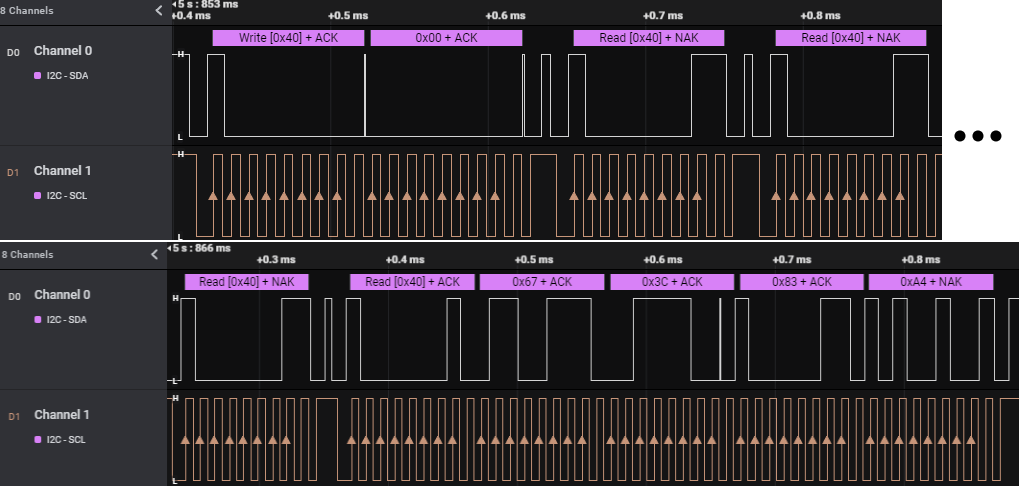
\includegraphics[scale=0.55]{figs/PI_HDC1080ReadOperation.png}
    \caption{Operatia de citire a temperaturii si a umiditatii}
    \label{fig:PI_HDC1080ReadOperation}
\end{figure}


{\color{blue}Împreună cu capitolul \textbf{precedent} și cel \textbf{următor} trebuie să reprezinte aproximativ 70\% din total.\\}

Scopul acestui capitol este de a documenta aplicația dezvoltată în așa fel încât dezvoltarea și întreținerea ulterioară să fie posibile.
Cititorul trebuie să identifice funcțiile principale ale aplicației din ceea ce este scris aici.
Capitolul ar trebui sa conțină (nu se rezumă neapărat la):
\begin{itemize}
	\item schema generală a aplicației
	\item descrierea fiecărei componente implementate, la nivel de modul
	\item diagrame de clase, clase importante și metode ale claselor importante.
    \item diagrame de baze de date
\end{itemize}
